% ==============
% PARAMETRAGES
% à compiler en pdfLaTeX
% ==============

% GENERAL
%  type de document rapport, chapitre commence en page impaire ou paire indifféremment
\documentclass[twoside,a4paper,11pt,frenchb,openany]{report}  
%  type de document, chapitre commence en page impaire
%\documentclass[twoside,a4paper,12pt,frenchb,openright]{report} 
\title{Rapport de stage}
\author{Stephane Robin}
\date{\today}

% IMPORTATION DE LIBRAIRIES
\usepackage{amssymb}  % symboles
\usepackage{amsmath}  % symboles mathématiques
\usepackage{amsfonts}  % polices de caractères
\usepackage{amscd}
\usepackage{amsthm}  % symboles mathématiques pour redéfinir les théorèmes
\usepackage[all,cmtip]{xy}
\usepackage{array}  % tableaux
\usepackage[frenchb]{babel}  % langue française
\usepackage{bm}  % caractères grecs
\usepackage{calc}
\usepackage[justification=centering]{caption} % centralise les légendes des figures
\usepackage{enumitem} % listes
\usepackage{eurosym}  % symbole euro
\usepackage{euscript}
\usepackage{fancybox}  % boîtes
\usepackage{float}  % images flottantes
\usepackage[T1]{fontenc}  % LaTeX modele
\usepackage[top=3.1cm,bottom=2.7cm,left=2.2cm,right=2.2cm,dvips]{geometry}  % marges
\usepackage{graphicx}  % insertion images
\usepackage[utf8]{inputenc}  % accents
\usepackage{mathrsfs}  % symboles mathématiques
\usepackage{mathtools}  % outils mathématiques
\usepackage{mdframed} % box autour des theoremes
\usepackage{pst-plot, pstricks}
\usepackage{pstricks-add}
\usepackage{rotating}
\usepackage{setspace} % permet de définir l'espace entre les lignes
\usepackage{srcltx}
\usepackage{textcomp}   % caracteres complementaires
\usepackage{titlesec}  % sections
\usepackage{titletoc}  % table de contents
%\usepackage[nottoc,notlof,notlot]{tocbibind}  % bibliothèque
\usepackage{verbatim}  % caracteres non interpretes
\usepackage{wrapfig}  % pour inserer les figures dans du texte

% COULEURS
\definecolor{couleurTitre}{RGB}{64,128,128}  % doit être défini avant xcolor
\definecolor{couleurUrl}{RGB}{127,62,0}
\usepackage{xcolor}  % couleurs
%\definecolor{amber}{rgb}{1.0,0.49,0.0} % couleur non utilisee
%\definecolor{greyish}{rgb}{52.0,160.0,157.0} % couleur non utilisee
%\definecolor{theoremeCouleur}{rgb}{224.0,90.0,67.0} % couleur non utilisee

% LISTES
\renewcommand{\labelitemi}{$\bullet$}  % symboles de listes
\frenchbsetup{StandardLists=true}  % style de bullets

% IMAGES
\usepackage{caption}  % insertion d'images
\usepackage[font=footnotesize,labelfont=bf]{caption}  % légendes des images
\renewcommand{\thefigure}{\arabic{figure}}  % numérotation des images
%\renewcommand{\thefigure}{\arabic{section}.\arabic{figure}}  % autre possibilité numérotation des images
\usepackage{subcaption}

% HYPERLINKS
\usepackage{hyperref}
\hypersetup{
	colorlinks=true,
	linkcolor=couleurUrl,
	citecolor=couleurUrl,
	urlcolor=couleurUrl,
	breaklinks=true % saute la ligne au milieu d'un href
}
\PassOptionsToPackage{hyphens}{url}\usepackage{hyperref} % pour que url ait les memes propriétés que hyperref

% LIGNES
\usepackage{parskip}
%\setlength\parskip{\baselineskip} % joint a la suppression de l'espace horizontal
%\setlength{\parindent}{0cm} % supprime l'espace horizontal en debut de ligne

% HEADINGS AND FOOTERS
\usepackage{fancyhdr}  % entete
\pagestyle{fancy}  % la page accepte les entetes et pieds de page
\renewcommand{\headrulewidth}{0pt}
\fancyhead[L,R,C]{}
%\fancyhead[LE]{} % pages paires header gauche
%\fancyhead[CE]{} % pages paires header centre
%\fancyhead[RE]{Le théorème de Pythagore} % pages paires header droit
%\fancyhead[LO]{Le théorème de Pythagore} % pages impaires header gauche
%\fancyhead[CO]{} % pages impaires header centre
%\fancyhead[RO]{} % pages impaires header droit
%\fancyfoot[c]{\textcolor{gray}{\thepage}}  % pied de page
%\fancyfoot[L,R,C]{} % forcing footer empty

% REDEFINITION DU STYLE DE THEOREM
\newmdtheoremenv[  % definitions
linewidth=5,
leftline=true,
rightline=false,
bottomline=false,
topline=false,
leftmargin=0,
rightmargin=0,
backgroundcolor=couleurTitre!20,
linecolor=orange!70,
innertopmargin=21pt,
skipabove=\topskip,
ntheorem=true]{definition}{Définition}

\newmdtheoremenv[  % theoremes
linewidth=5,
leftline=true,
rightline=false,
bottomline=false,
topline=false,
leftmargin=0,
rightmargin=0,
backgroundcolor=couleurTitre!20,
linecolor=orange!70,
innertopmargin=10pt,
skipabove=\topskip,
ntheorem=true]{theorem}{}

\newmdtheoremenv[  % proprietes
linewidth=5,
leftline=true,
rightline=false,
bottomline=false,
topline=false,
leftmargin=0,
rightmargin=0,
backgroundcolor=couleurTitre!20,
linecolor=orange!70,
innertopmargin=21pt,
skipabove=\topskip,
ntheorem=true]{property}{Propriété}

\newmdtheoremenv[  % propositions
linewidth=5,
leftline=true,
rightline=false,
bottomline=false,
topline=false,
leftmargin=0,
rightmargin=0,
backgroundcolor=couleurTitre!20,
linecolor=couleurTitre!70,
innertopmargin=21pt,
skipabove=\topskip,
ntheorem=true]{proposition}{Proposition}

\newmdtheoremenv[  % corollaires
linewidth=5,
leftline=true,
rightline=false,
bottomline=false,
topline=false,
leftmargin=0,
rightmargin=0,
backgroundcolor=couleurTitre!20,
linecolor=couleurTitre!70,
innertopmargin=21pt,
skipabove=\topskip,
ntheorem=true]{corollary}{Corollaire}

\newmdtheoremenv[  % lemmes
linewidth=5,
leftline=true,
rightline=false,
bottomline=false,
topline=false,
leftmargin=0,
rightmargin=0,
backgroundcolor=couleurTitre!20,
linecolor=couleurTitre!70,
innertopmargin=21pt,
skipabove=\topskip,
ntheorem=true]{lemma}{Lemme}

% NUMEROTATION DES CHAPITRES-SECTIONS
\renewcommand{\theequation}{\arabic{chapter}.\arabic{equation}}  % equations
%\renewcommand{\theequation}{\thesection\arabic{equation}}  % equations
%\numberwithin{equation}{section}  % equations

%\renewcommand{\thepart}{\Alph{part}}  % parties
%\renewcommand{\thechapter}{\arabic{chapter}.}  % chapitres
\renewcommand{\thesection}{\arabic{section}.}  % sections
\renewcommand{\thesubsection}{\arabic{section}.\arabic{subsection}.}  %  sous-sections
\renewcommand{\thesubsubsection}{\arabic{section}.\arabic{subsection}.\arabic{subsubsection}.}  % sous-sous-sections

\renewcommand{\thedefinition}{\arabic{chapter}.\arabic{definition}}  % definitions
\renewcommand{\theorem}{}  % theoremes
\renewcommand{\theproperty}{\arabic{chapter}.\arabic{property}}  % property
\renewcommand{\theproposition}{\arabic{chapter}.\arabic{proposition}}  % propositions
\renewcommand{\thecorollary}{\arabic{chapter}.\arabic{corollary}}  % corollaires
\renewcommand{\thelemma}{\arabic{chapter}.\arabic{lemma}}  % lemmes
\setcounter{secnumdepth}{4}  % profondeur de numérotation

% FORMAT DES SECTIONS-TITRES
\titleformat{\section}{\normalfont\normalsize\bfseries}{\textcolor{couleurTitre}{\thesection}}{1.2em}
{\normalfont\large\bfseries\scshape\textcolor{couleurTitre}} % format de titre de section
\titleformat{\subsection}{\normalfont\normalsize\bfseries}{\textcolor{couleurTitre}{\thesubsection}}{1em}
{\normalfont\normalsize\bfseries\textcolor{couleurTitre}}  % format de titre de sous-section
\titleformat{\subsubsection}{\normalfont\normalsize\bfseries\itshape}{\textcolor{couleurTitre}{\thesubsubsection}}{1em}
{\normalfont\normalsize\bfseries\itshape\textcolor{couleurTitre}}  % format de titre de sous-sous-section

\makeatletter

% CONCERNE LA TABLE DES MATIERES
%\renewcommand{\@chapapp}{}  % le mot `chapitre'' n'apparait plus en titre de chapitre
\renewcommand\l@section{\@dottedtocline{1}{0em}{1.5em}}  % espacement dans le titre d'une section
\renewcommand\l@subsection{\@dottedtocline{1}{2.5em}{2.5em}}  % espacement dans le titre d'une sous-section
\renewcommand\l@subsubsection{\@dottedtocline{1}{5em}{2.5em}}  % espacement dans le titre d'une sous-sous-section

\makeatother

% ==============
% DEBUT DU DOCUMENT
% ==============

\begin{document}
	
	\maketitle
	
	\tableofcontents
	
	
	% REMERCIEMENTS ----------------------------
	
	\section{Remerciements}
	
	
	% INTRODUCTION --------------------------------
	
	\section{Introduction}
	Les objectifs du projet. Le caractère hands-on et complet.


	% ETAT DE L'ART -------------------------------------
	\section{Etat de l'art}


	

% CHOIX DES OUTILS -----------------------------
\section{Le choix des outils}

Définissons tout d'abord le vocabulaire que nous allons utiliser dans ce rapport de stage :
\begin{itemize}
\item module : un fichier contenant du code Python,
\item package : un répertoire contenant des modules Python,
\item distribution : une archive de modules ou packages (au format tar, whl, ...)
\end{itemize}


% CHOIX DE L'ENVIRONNEMENT DE TRAVAIL -----------------------------

\subsection{Choix de l'environnement de développement}

Afin de tester les codes de ce projet, l'outil de création d'environnement virtuel \textit{venv} nous permet de créer un environnement de développement. \textit{venv} constitue en fait un dossier contenant tous les exécutables nécessaires pour utiliser les modules d'un projet Python.

Par ailleurs, le module \textit{pyenv} nous permet de définir une version de Python comme version locale de travail dans cet environnement. Nous choisissons Python 3.6.5.

Finalement, nous installons dans cet environnement les dépendances nécessaires à l'aide de l'outil \textit{pip} :
\begin{itemize}
\item pkg-resources==0.0.0 (installé automatiquement)
\item pip install xmltodict : le module xmltodict permet de lire du code XML comme si il s'agissait de code JSON. Il permet donc une lecture plus rapide des fichiers.
\item subprocess.run==0.0.8\\
Le module subprocess permet de gérer de nouveaux processus, de se connecter à leurs flux d'input/output/erreurs. Il remplace plusieurs modules dépréciés : os. system, os.spawn*, os.popen*, popen2.*, commands.* 
\item pip install openpyxl : le package openpyxl permet de lire et d'écrire dans des fichiers Excel de type xlsx, xlsm, xltx, xltm. Il comprend les modules et-xmlfile et jdcal.
\item pip install xlrd : le module xlrd extrait des données d'un tableur Excel à partir de la version 2.0 et avant de les formatte.
\item pip install biopython : le package biopython regroupe un ensemble d'outils Python pour le traitement informatique de la biologie moléculaire et comprend le module numpy.
\item DateTime==4.3\\
Le module datetime permet de manipuler des dates et heures en gérant des objets de type DateTime. 
\item pytz==2019.3 (installé avec le module datetime)
\item zope.interface==5.0.1 (installé avec le module datetime)
\end{itemize}

En outre, certains modules sont déjà présents dans le package standard Python3 :
\begin{itemize}
\item le module os fournit une manière portable d'utiliser les fonctionnalités dépendantes du système d'exploitation,
\item le module pickle permet de sérialiser et désérialiser une structure d'objet Python. Il remplace le module primitif marshal. pickle se trouve déjà dans la librairie standard Python3,
\item le module csv implémente des classes pour lire et écrire des données liées à des feuilles de calcul ou des bases de données au format csv,
\item le module shutil propose des opérations sur les fichiers et collections de fichiers, notamment la copie et suppression de fichiers.
\end{itemize}

Notre package, une fois créé, devrait proposer le même environnement de travail et donc contenir ces mêmes modules.
 

% COMPOSITION D'UN PACKAGE STANDARD ------------------
	
\subsection{Composition d'un package standard}

Un package standard comporte obligatoirement un fichier \_\_init\_\_.py qui va définir la version du projet et le nom du module de lancement du programme (souvent \_\_main\_\_.py).

Les fichiers setup.py,  requirements.txt, LICENSE et README.md sont également nécessaires.  
\begin{itemize}
\item setup.py est le script de construction destiné à setuptools. Il définit le nom et la version du package, ainsi que les fichiers qu'il contient. 
\item requirements.txt permet l'installation des dépendances à l'aide d'un unique fichier contenant un module à installer par ligne. Il nécessite l'instruction pour commencer ces installations.
\item LICENSE définit 
\item README.md décrit l'installation du package, la nature de ses dépendances et les principales fonctionnalités.
\end{itemize}

Avec la PEP-518, le PyPA a proposé un nouveau standard au format package.toml, qui remplace les fichiers setup.py, requirements.txt, setup.cfg, MANIFEST.in et Pipfile. C'est ce nouveau standard qui est utilisé lors de la création d'un package avec Poetry.

La commande poetry new nomPaquet permet de générer le squelette de l'application, comprenant les tests unitaires, le fichier pyproject.toml, le fichier README.rst que nous changeons au format markdown README.md, le répertoire du projet et le fichier init.py. Nous rajoutons un fichier LICENSE, les composants principaux de la librairie, le présent rapport de stage et un fichier .gitignore pour la gestion des versions.
	
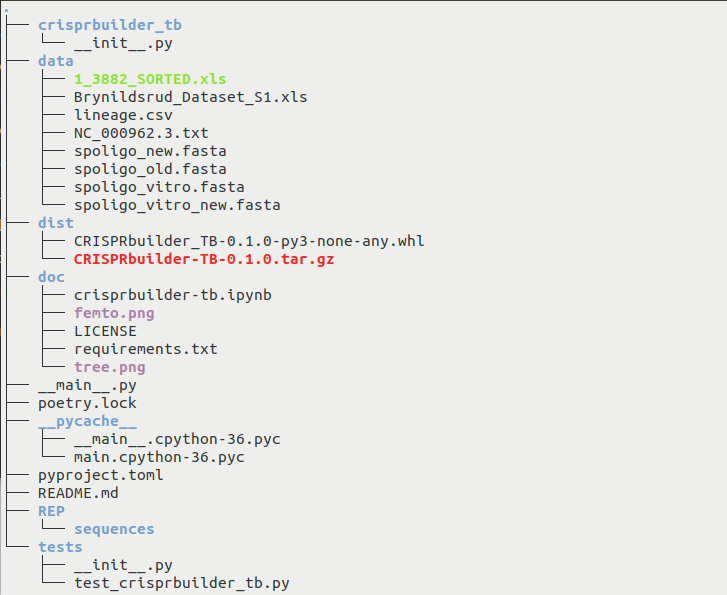
\includegraphics[width=5cm]{package_tree.png}

	La plupart des systèmes d'exploitation incorporent Python2.7 par défaut. L'environnement de travail devra donc expressément définir Python3 comme version pour le projet. Nous avons choisi la version 3.6.5 de Python dans le fichier package\_mymtc.toml.

Les paquets construits pour des systèmes Unix (Linux et MacOS) nécessitent l'incorporation de fichiers build.sh et meta.yaml. Les paquets construits pour les systèmes Windows nécessitent l'incorporation des fichiers bld.bat et meta.yaml. A VERIFIER DANS LE CAS DE POETRY


% QUELLE LICENCE CHOISIR ------------------
\subsection{Quelle licence choisir ?}
	
Trois licences retiennent notre attention. En voici les principales caractéristiques :
\begin{itemize}
\item	la licence MIT, courte et permissive, préserve exclusivement le copyright et les avis de licence. Toute modification ultérieure peut être distribuée suivant une licence différente et notamment utilisée à des fins personnelles ou commerciales, sans obligation de publication des codes source,
\item	la licence Apache (2.0) est également permissive et sensiblement similaire dans ses conditions à la licence MIT. Toutefois, elle requiert de préciser les modifications effectuées lors de nouvelles distributions,
\item	la licence GNU (GPL v3.0) préserve également le copyright et les avis de licence. Elle peut être utilisée à des fins personnelles et commerciales. Elle impose en outre, en cas de modification, la publication complète des codes et l'utilisation de la licence GNU pour les nouvelles distributions.
\end{itemize}

Nous choisissons la licence MIT qui semble répondre aux besoins de ce projet.

	

	% CHOIX DE L'OUTIL D'EMPAQUETAGE --------------------
	
	\subsection{Choix de l'outil d'empaquetage}
	
	Le PyPA \textit{Python Packaging User Guide} recommande l'utilisation de :
\begin{itemize}
\item \textit{pip} pour l'installation de librairies à partir de PyPI \textit{Python Package Index},
\item \textit{setuptools} pour définir des projets et créer des sources de distribution,
\item \textit{pipenv} pour la gestion des dépendances de librairies lors de développement d'applications Python,
\item \textit{venv} pour isoler les dépendances particulières d'une application,
\item \textit{conda} pour les projets scientifiques.
\item \textit{buildout} pour les projets de développement Web,
\item \textit{poetry} pour un besoin particulier non couvert par Pipenv.
\end{itemize}
	
\textit{pipenv} est un gestionnaire de haut niveau pour les environnements, les dépendances et les packages Python. Contrairement à \textit{virtualenv}, \textit{pipenv} distingue les dépendances du projet et les dépendances des dépendances du projet. Par ailleurs, \textit{pipenv} différencie le mode développement du mode production. Il offre l'avantage de bien fonctionner sur Windows. Toutefois, la communauté Python l'a peu mis à jour depuis 2018.

\textit{Anaconda} est une distribution de logiciels multiplateformes (Windows, Linux, MacOS) qui facilite l'installation des librairies scientifiques \textit{Numpy} et \textit{Scipy}, ce qui est particulièrement intéressant dans le cas des plateformes Windows où ce processus est plus complexe. Elle incorpore une librairie open-source appelée conda permettant la gestion des dépendances, de l'environnement de travail ainsi que la création de packages. \textit{Anaconda} semble être approprié au projet, mais c'est une distribution trop lourde pour être intégrée à notre package et \textit{Miniconda}, qui ne comporte que Python, conda et pip, ne répond pas au besoin du projet.

Nous avons naturellement cherché à construire le package manuellement, à partir de pipenv puis de conda. Cet effort s'est avéré laborieux et a révélé des incompatibilités qui n'ont pas permis de valider les exigences de la plateforme testPyPI.

Nous avons donc décidé de construire notre package en utilisant \textit{poetry}, qui est un outil complet autour duquel la communauté Python reste très active. Il propose à la fois la gestion des dépendances, l'empaquetage (création d'une structure pour un projet et la génération de fichiers de configuration et de manifestes) et la publication.

	



% LA STRUCTURE D'UN PACKAGE SOUS POETRY

\subsection{La structure d'un package sous Poetry}


 
\subsection{L'outil de création de package et gestion des dépendances \textit{Poetry}}


	% LA COMPOSITION DU PACKAGE ------------------------
	
	\section{La composition du package}

Le package est décrit dans le document .md













% CREATION DE LA LIBRAIRIE --------------------------------

\section{La création de la librairie}

=== A CHANGER ===
Pour créer une librairie à partir de conda, il est nécessaire d'installer conda-build puis de construire un recipe composé de :
\begin{itemize}
\item un fichier meta.yaml contenant toutes les métadata du recipe
\item un script build.sh qui installe les fichiers de la librairie sur Linux et macOS, exécuté avec une commande bash
\item un script bld.bat qui installe les fichiers de la librairie sur Windows, exécuté avec une commande cmd
\item un fichier optionnel $run_test.py$, qui s'exécute automatiquement pour effectuer des tests
\item un fichier readme et des icônes si nécessaire.  
\end{itemize}
Les trois premiers fichiers se créent avec la commande conda skeleton.
===FIN CHANGEMENT===




	
	

	

% LES ELEMENTS DU CODE ------------------------------------------

\section{Les principaux éléments du code}

dico est composé de la façon suivante :

Un fichier pkl tel que dico\_africanum.pkl est créé par pickle et contient un flux d'octets représentant les objets à sérialiser.

pickle permet aux objets d'être sérialisés en fichiers sur disque et désérialisés dans le programme au moment de l'exécution.
	
	% =========
	% BIBLIOTHEQUE
	% =========
	\begin{spacing}{0.5}
		\bibliographystyle{}
		\renewcommand{\bibname}{Références}
		\begin{thebibliography}{10}
			\href{https://packaging.python.org/guides/}{https://packaging.python.org/guides/}\\

\href{https://realpython.com/pypi-publish-python-package/}{https://realpython.com/pypi-publish-python-package/}
			
		\end{thebibliography}
	\end{spacing}
\end{document}
